\begin{figure}[h!]
    \centering
    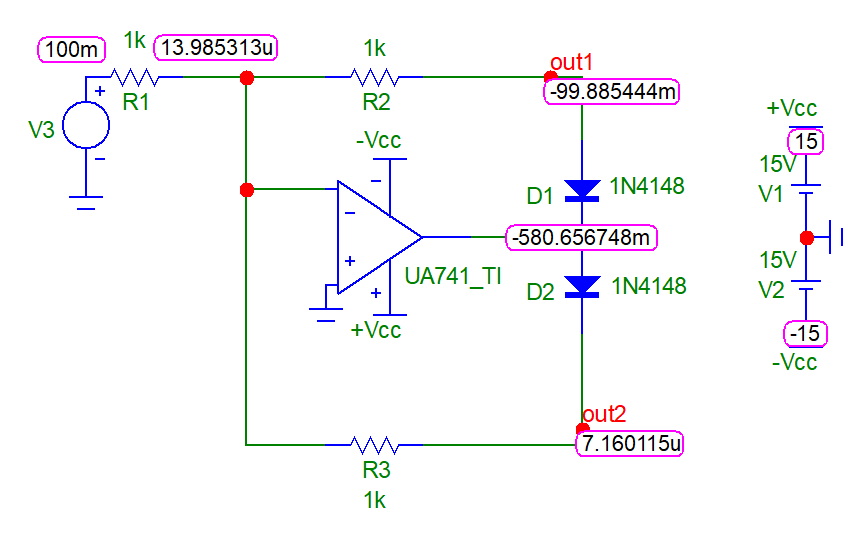
\includegraphics[width=0.63\textwidth]{microcap/1-dcbod.png}
    \caption{Zapojení a) -- stejnosměrný prac. bod pro kladné vstupní napětí.}
    \label{fig:microcap/.png}
\end{figure}

\begin{figure}[h!]
    \centering
    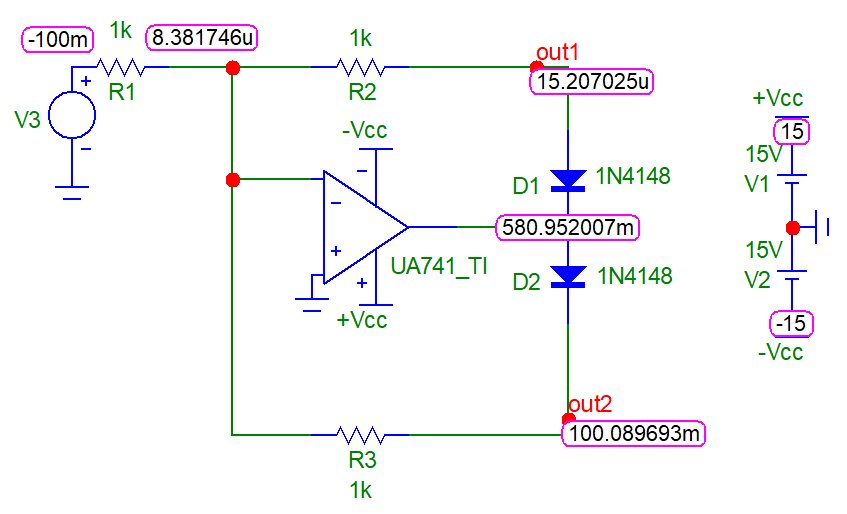
\includegraphics[width=0.63\textwidth]{microcap/1-dcbod2.png}
    \caption{Zapojení a) -- stejnosměrný prac. bod pro záporné vstupní napětí.}
    \label{fig:microcap/.png}
\end{figure}

\begin{figure}[h!]
    \centering
    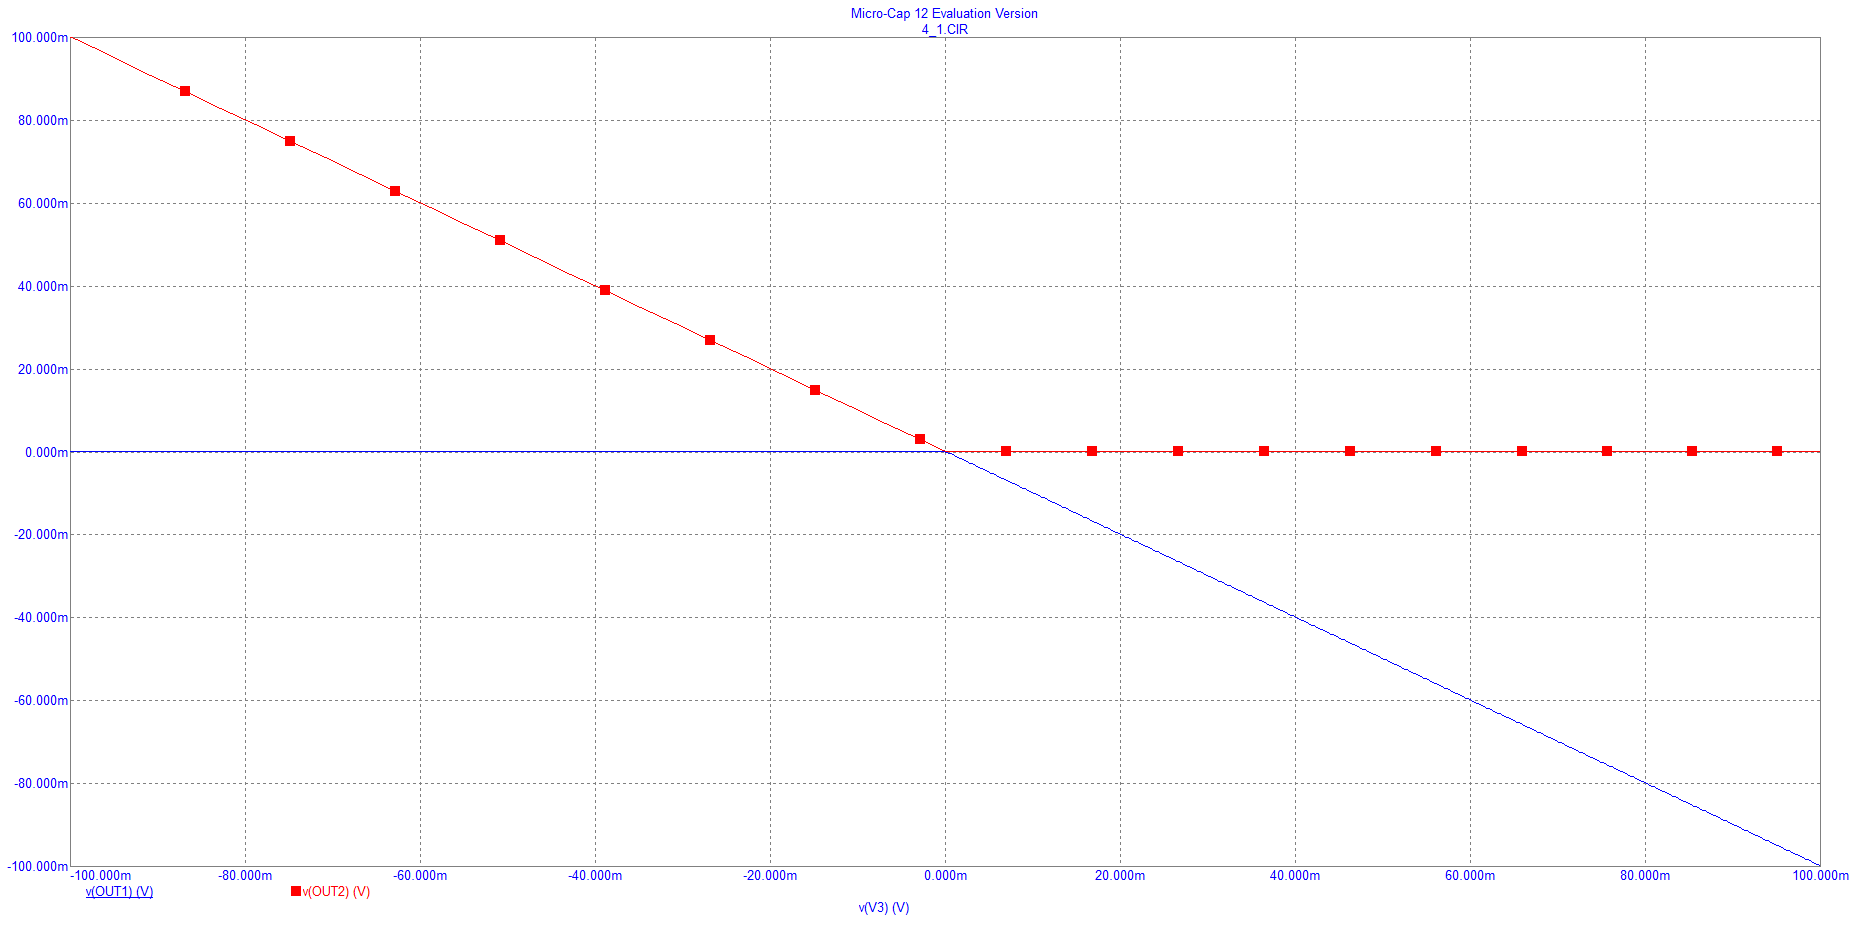
\includegraphics[width=0.8\textwidth]{microcap/1-dcprevodni.png}
    \caption{Zapojení a) -- stejnosměrná převodní charakteristika.}
    \label{fig:microcap/.png}
\end{figure}

\begin{figure}[h!]
    \centering
    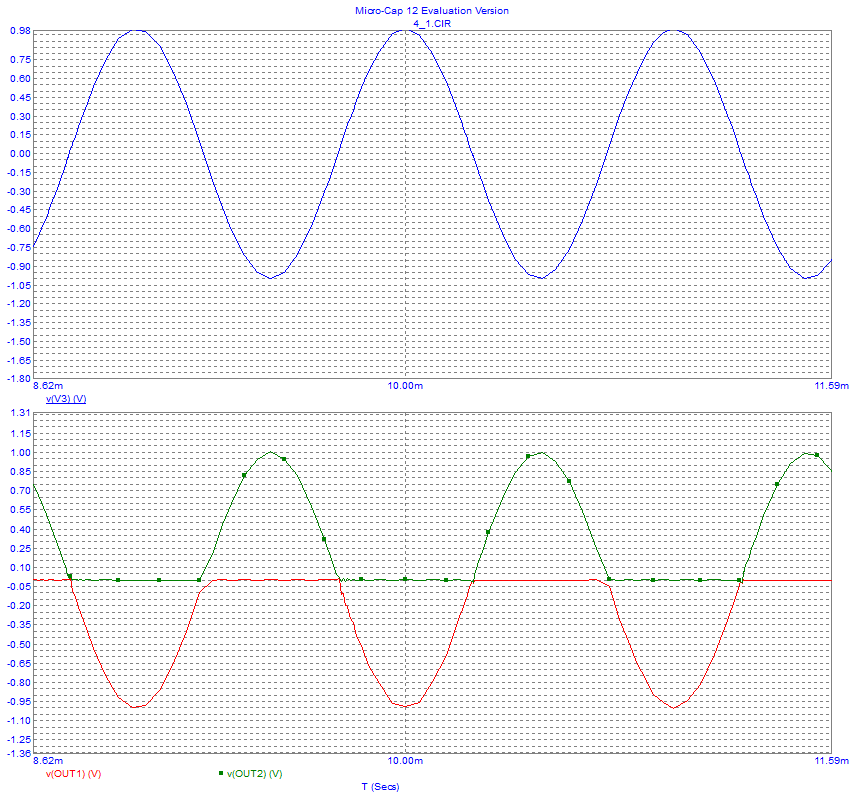
\includegraphics[width=0.8\textwidth]{microcap/1-transient-1khz-1v.png}
    \caption{Zapojení a) -- časová závislost obou výstupních napětí na vstupním napětí, jednocestné zesílení, \(f=\qty{1}{\kilo\hertz}, U_M=\qty{1}{\volt}\).}
    \label{fig:microcap/.png}
\end{figure}

\begin{figure}[h!]
    \centering
    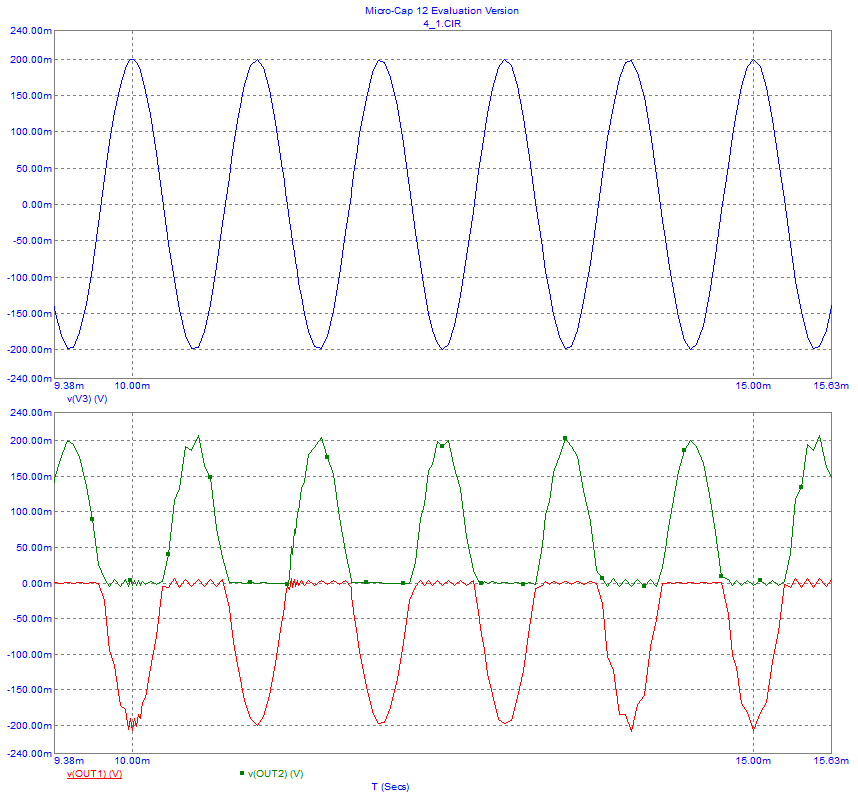
\includegraphics[width=0.7\textwidth]{microcap/1-transient-1khz-0.2v.png}
    \caption{Zapojení a) -- časová závislost obou výstupních napětí na vstupním napětí, nejmenší amplituda, při které zapojení obstojně usměrňuje, \(f=\qty{1}{\kilo\hertz}, U_M=\qty{200}{\milli\volt}\).}
    \label{fig:microcap/.png}
\end{figure}

\begin{figure}[h!]
    \centering
    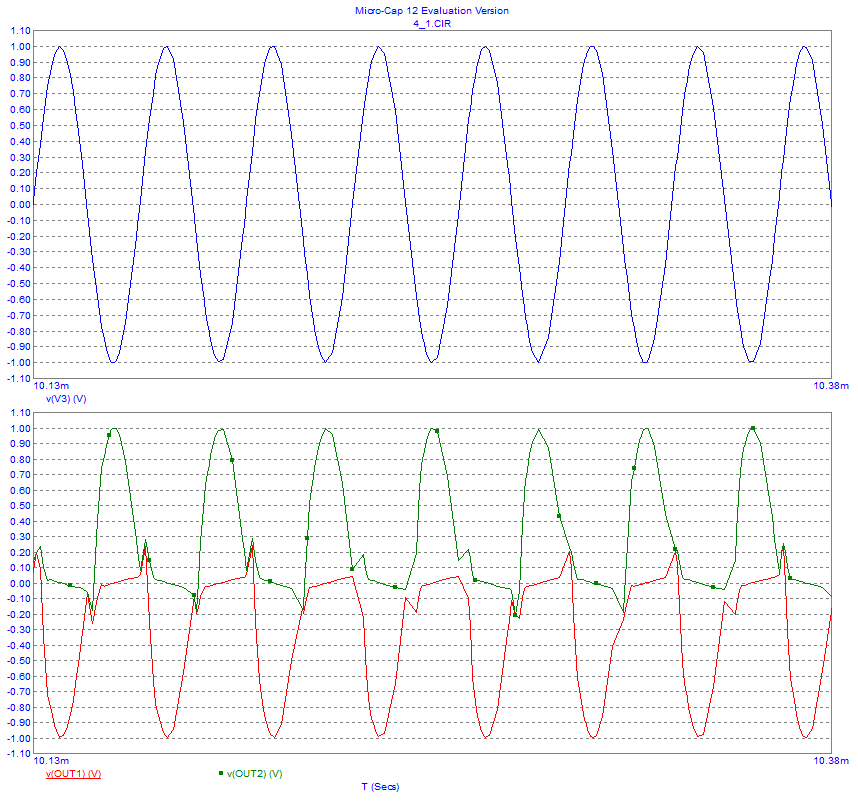
\includegraphics[width=0.7\textwidth]{microcap/1-transient-30khz-1v.png}
    \caption{Zapojení a) -- časová závislost obou výstupních napětí na vstupním napětí, nejvyšší frekvence, při které zapojení obstojně usměrňuje, \(f=\qty{30}{\kilo\hertz}, U_M=\qty{1}{\volt}\).}
    \label{fig:microcap/.png}
\end{figure}

\begin{figure}[h!]
    \centering
    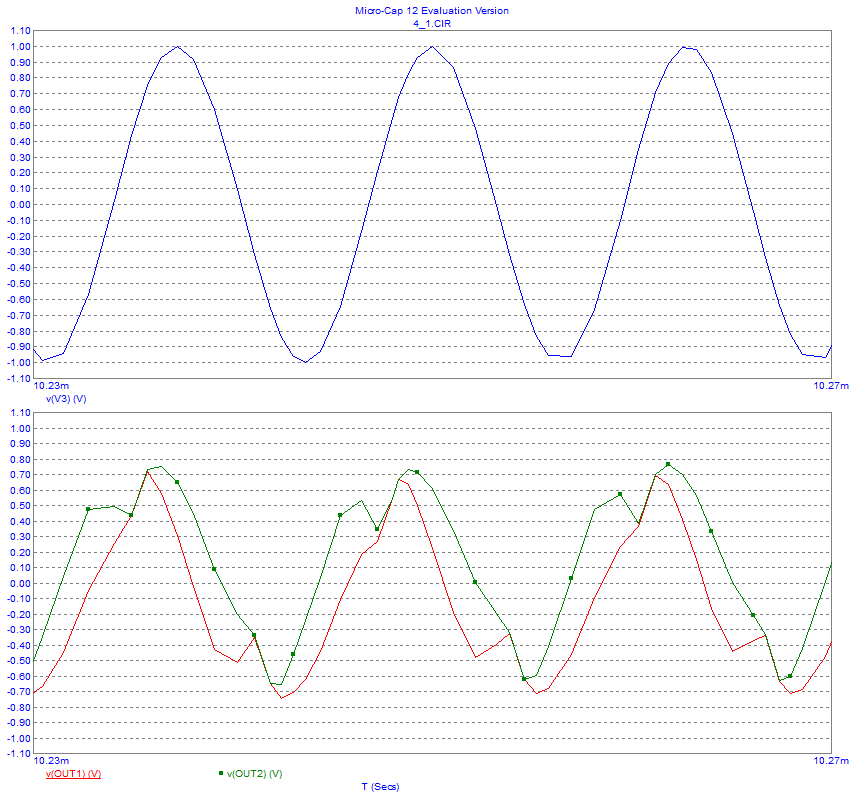
\includegraphics[width=0.8\textwidth]{microcap/1-transient-100khz-1v.png}
    \caption{Zapojení a) -- časová závislost obou výstupních napětí na vstupním napětí, příliš vysoká frekvence, k usměrnění nedochází vůbec, \(f=\qty{100}{\kilo\hertz}, U_M=\qty{1}{\volt}\).}
    \label{fig:microcap/.png}
\end{figure}    

% \begin{figure}[h!]
%     \centering
%     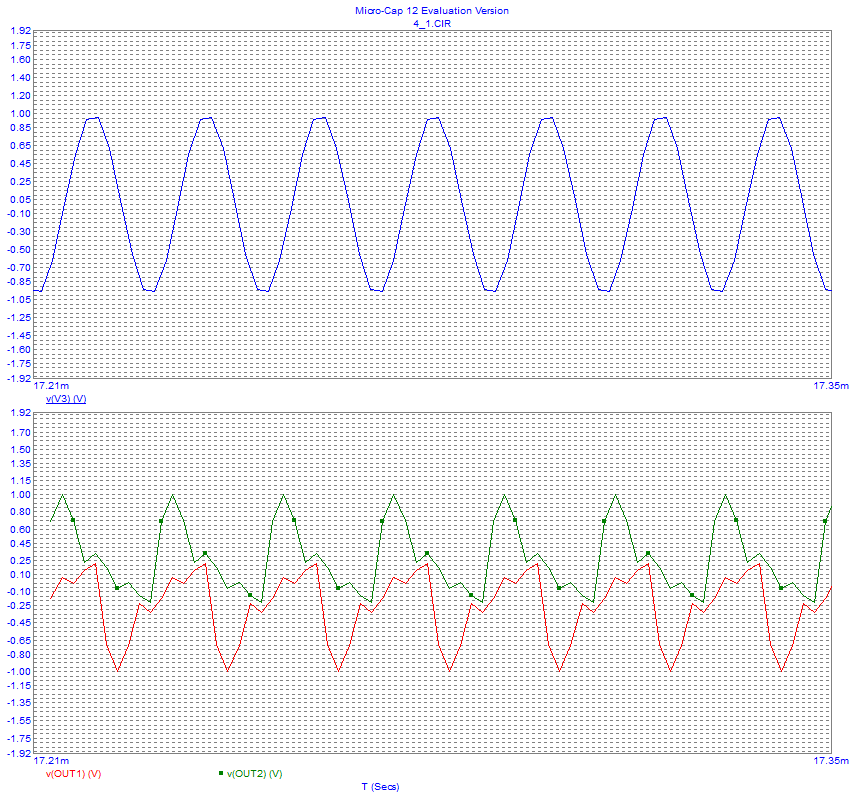
\includegraphics[width=0.8\textwidth]{microcap/1-transient-50khz-1v.png}
%     \caption{microcap/.png}
%     \label{fig:microcap/.png}
% \end{figure}

\begin{figure}[h!]
    \centering
    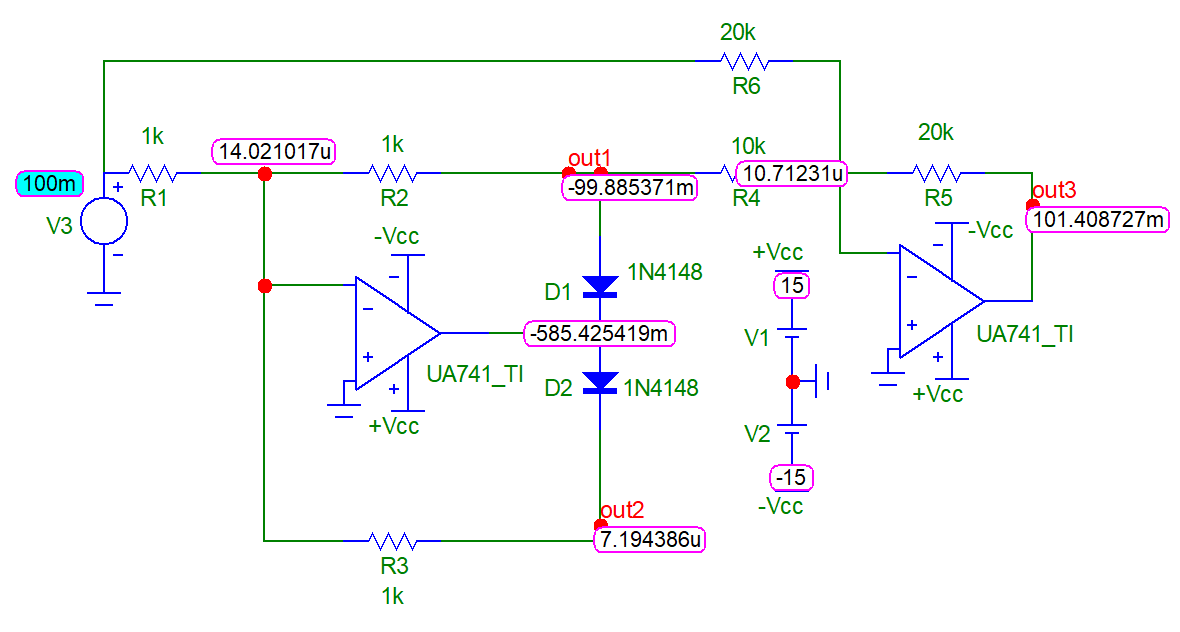
\includegraphics[width=0.8\textwidth]{microcap/2-dcbod.png}
    \caption{Zapojení b) -- stejnosměrný prac. bod při kladném napětí na vstupu, na výstupu kladné napětí.}
    \label{fig:microcap/.png}
\end{figure}

\begin{figure}[h!]
    \centering
    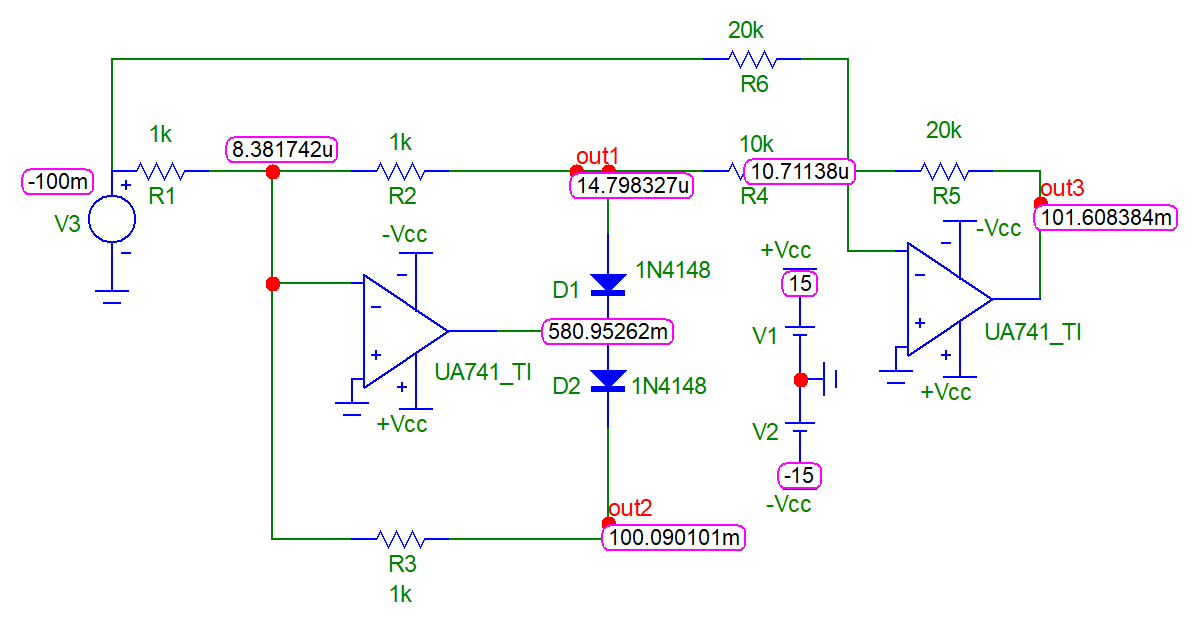
\includegraphics[width=0.61\textwidth]{microcap/2-dcbod2.png}
    \caption{Zapojení b) -- stejnosměrný prac. bod při záporném napětí na vstupu, na výstupu opět kladné napětí.}
    \label{fig:microcap/.png}
\end{figure}

\begin{figure}[h!]
    \centering
    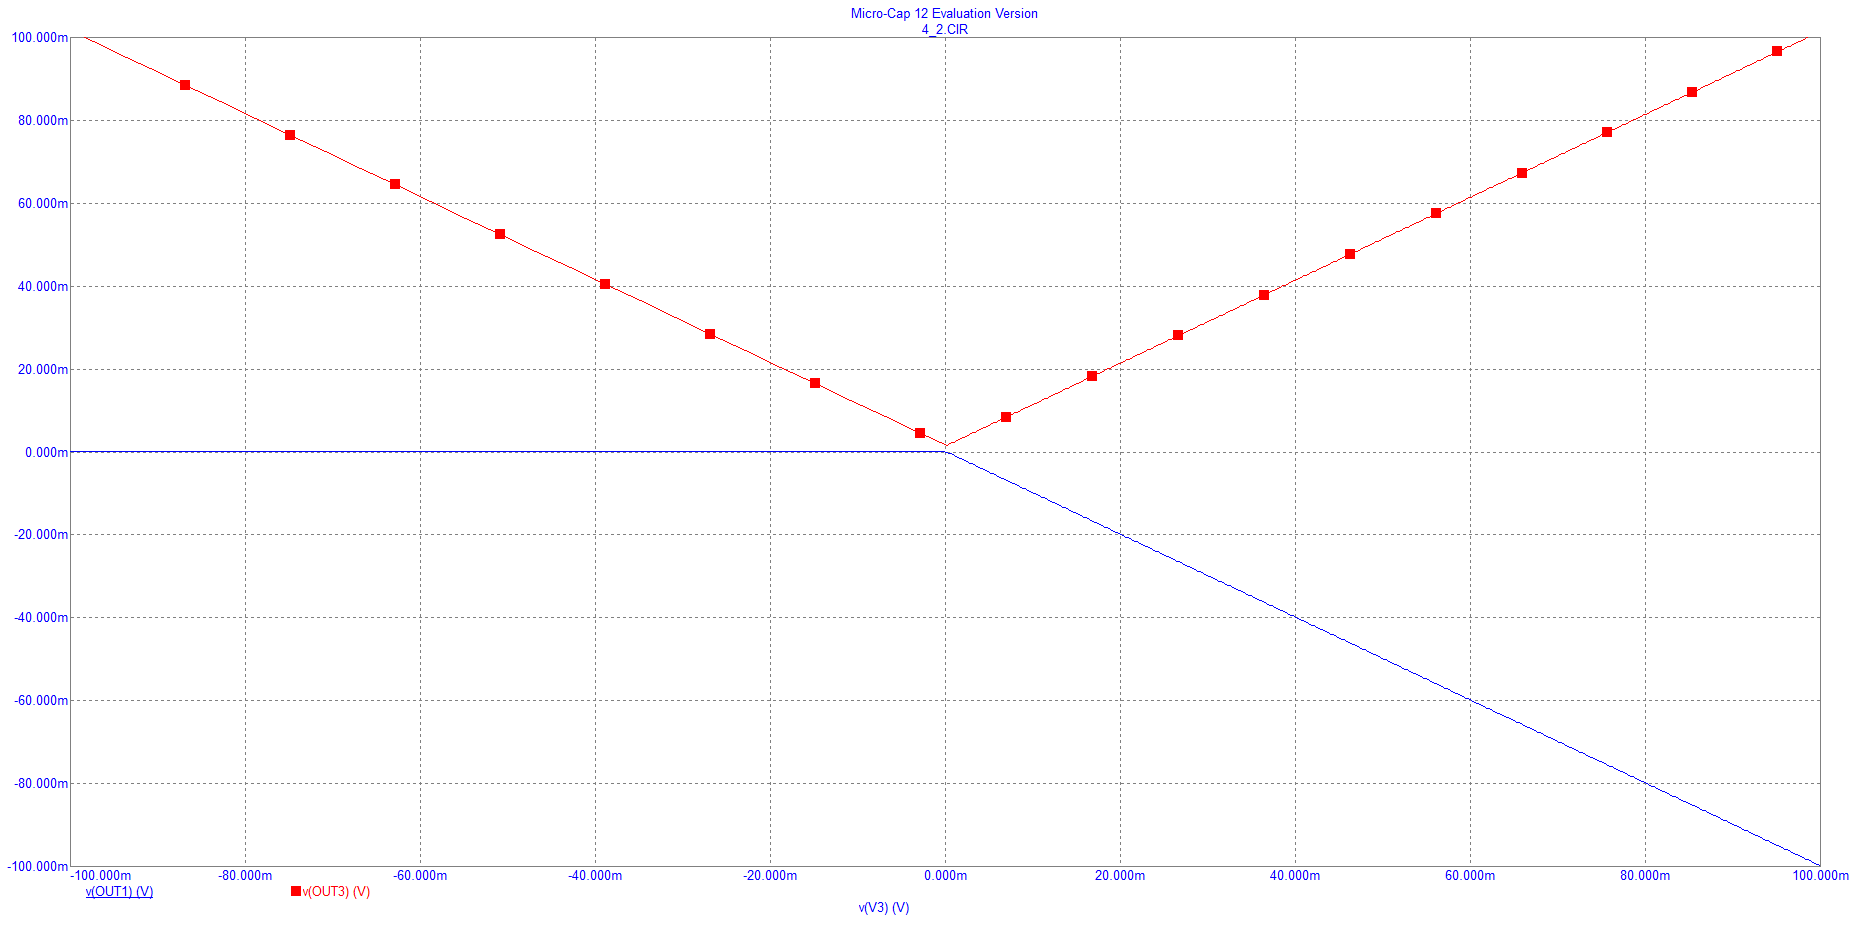
\includegraphics[width=0.61\textwidth]{microcap/2-dcprevodni.png}
    \caption{Zapojení b) -- stejnosměrná převodní charakteristika dvoucestného usměrnění.}
    \label{fig:microcap/.png}
\end{figure}

\begin{figure}[h!]
    \centering
    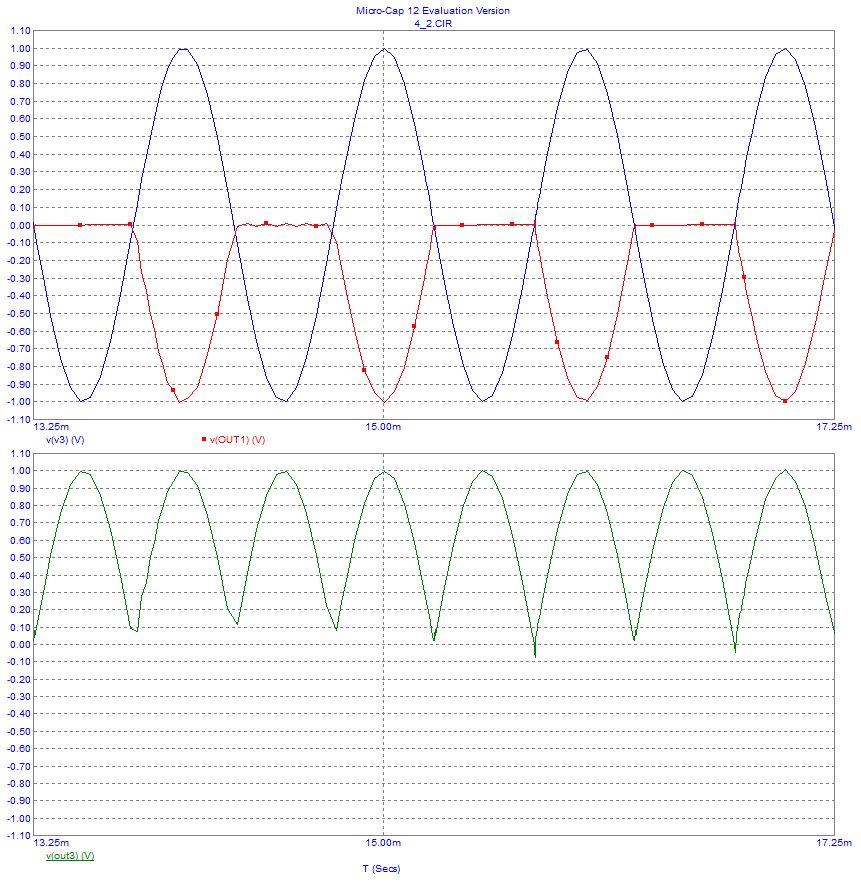
\includegraphics[width=0.61\textwidth]{microcap/2-transient-1khz-1v.png}
    \caption{Zapojení b) -- časová závislost napětí na výstupech obou OZ na vstupním napětí, jednocestné a dvoucestné usměrnění, \(f=\qty{1}{\kilo\hertz}, U_M=\qty{1}{\volt}\).}
    \label{fig:microcap/.png}
\end{figure}

% \begin{figure}[h!]
%     \centering
%     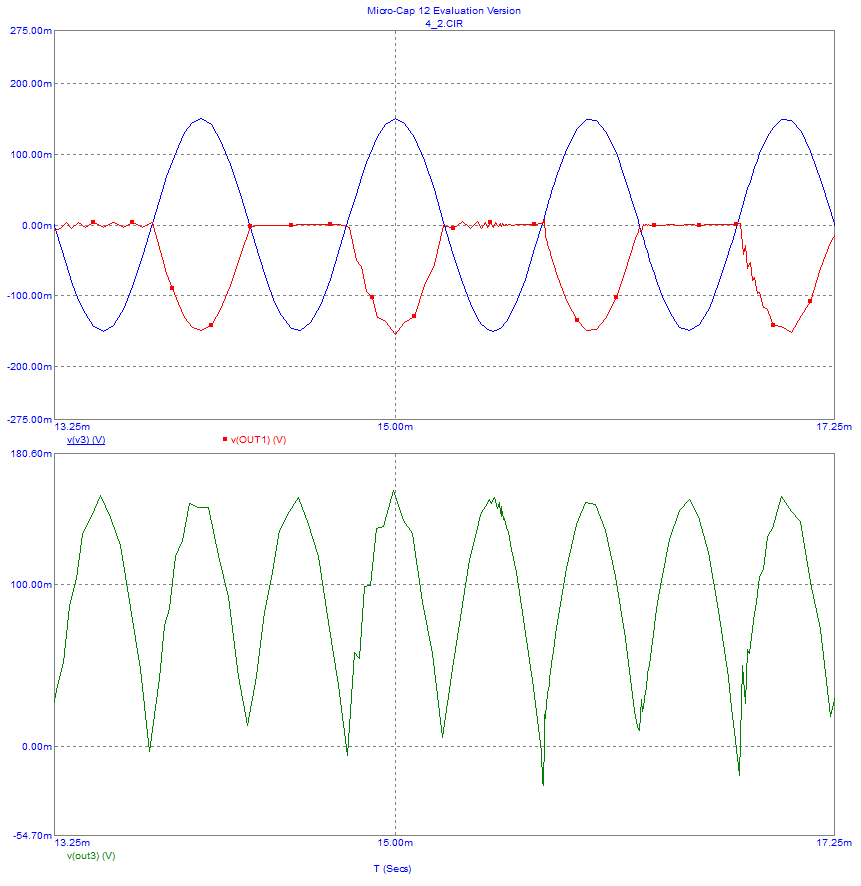
\includegraphics[width=0.8\textwidth]{microcap/2-transient-1khz-0.15v.png}
%     \caption{Zapojení b) -- časová závislost napětí na výstupech obou OZ na vstupním napětí, nejmenší amplituda, při které uspokojivě usměrňuje, \(f=\qty{1}{\kilo\hertz}, U_M=\qty{150}{\milli\volt}\).}
%     \label{fig:microcap/.png}
% \end{figure}

\begin{figure}[h!]
    \centering
    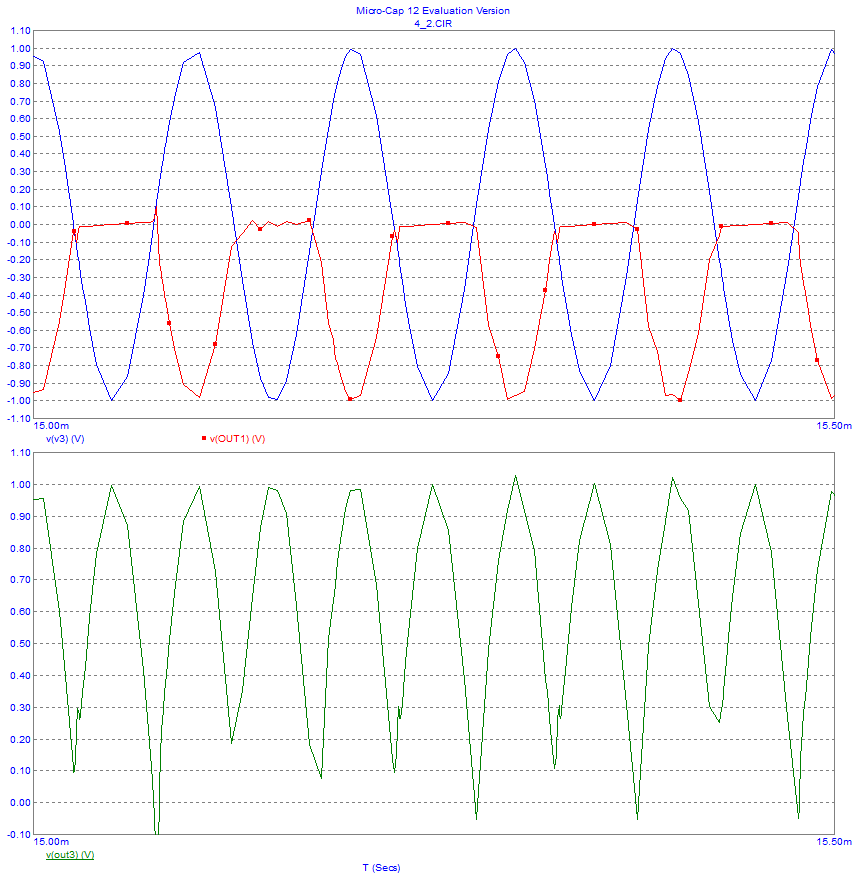
\includegraphics[width=0.7\textwidth]{microcap/2-transient-10khz-1v.png}
    \caption{Zapojení b) -- časová závislost napětí na výstupech obou OZ na vstupním napětí, nejvyšší frekvence, při které uspokojivě usměrňuje, \(f=\qty{10}{\kilo\hertz}, U_M=\qty{1}{\volt}\).}
    \label{fig:microcap/.png}
\end{figure}

\begin{figure}[h!]
    \centering
    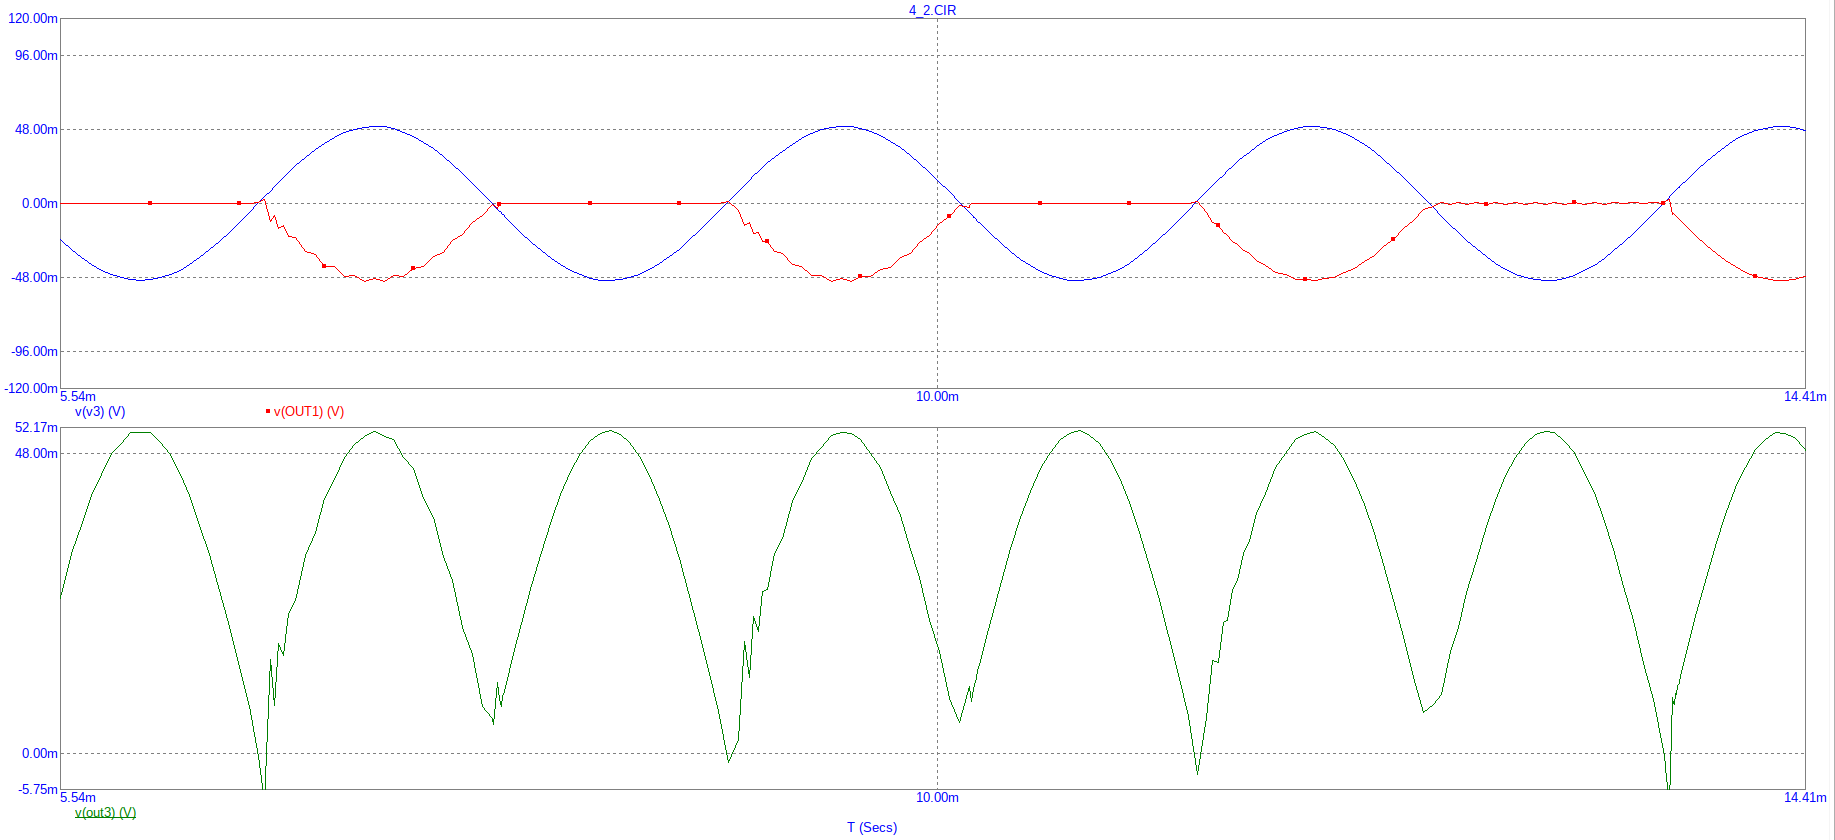
\includegraphics[width=0.7\textwidth]{microcap/2-transient-420hz-0.05v.png}
    \caption{Zapojení b) -- časová závislost napětí na výstupech obou OZ na vstupním napětí, nejnižší amplituda, při které uspokojivě usměrňuje, \(f=\qty{420}{\hertz}, U_M=\qty{50}{\milli\volt}\).}
    \label{fig:microcap/.png}
\end{figure}

\begin{figure}[h!]
    \centering
    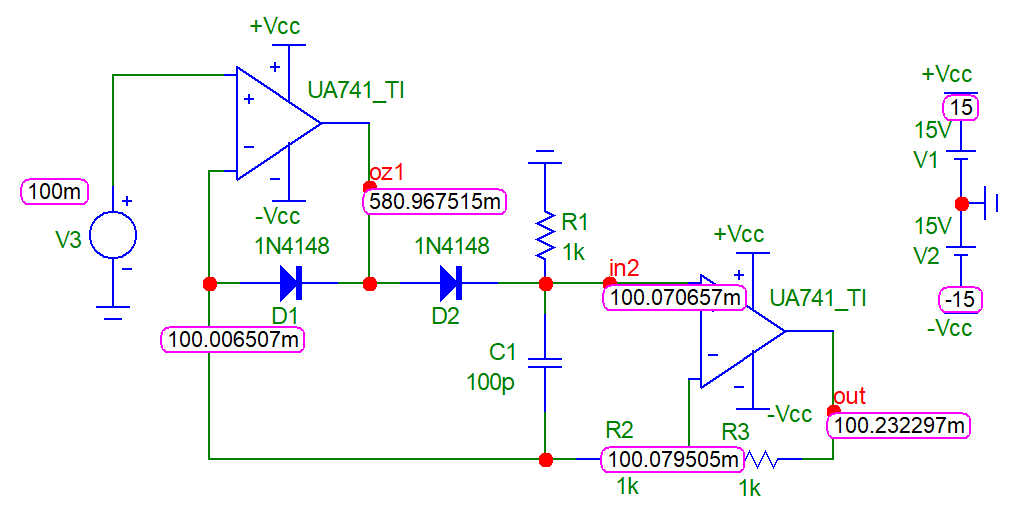
\includegraphics[width=0.8\textwidth]{microcap/3-dcbod.png}
    \caption{Zapojení c) -- stejnosměrný prac. bod při kladném napětí na vstupu, na výstupu kladné napětí.}
    \label{fig:microcap/.png}
\end{figure}

\begin{figure}[h!]
    \centering
    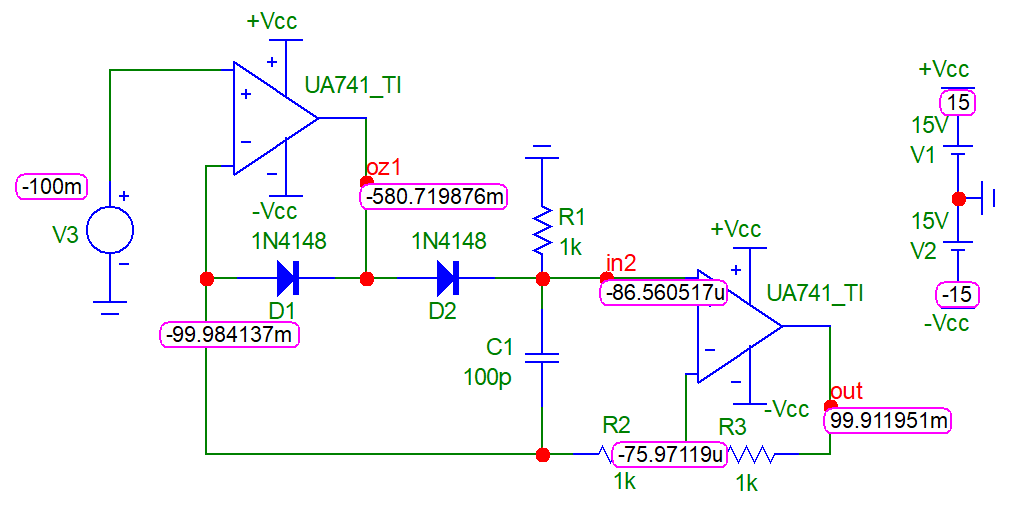
\includegraphics[width=0.8\textwidth]{microcap/3-dcbod2.png}
    \caption{Zapojení c) -- stejnosměrný prac. bod při záporném napětí na vstupu, na výstupu kladné napětí.}
    \label{fig:microcap/.png}
\end{figure}

\begin{figure}[h!]
    \centering
    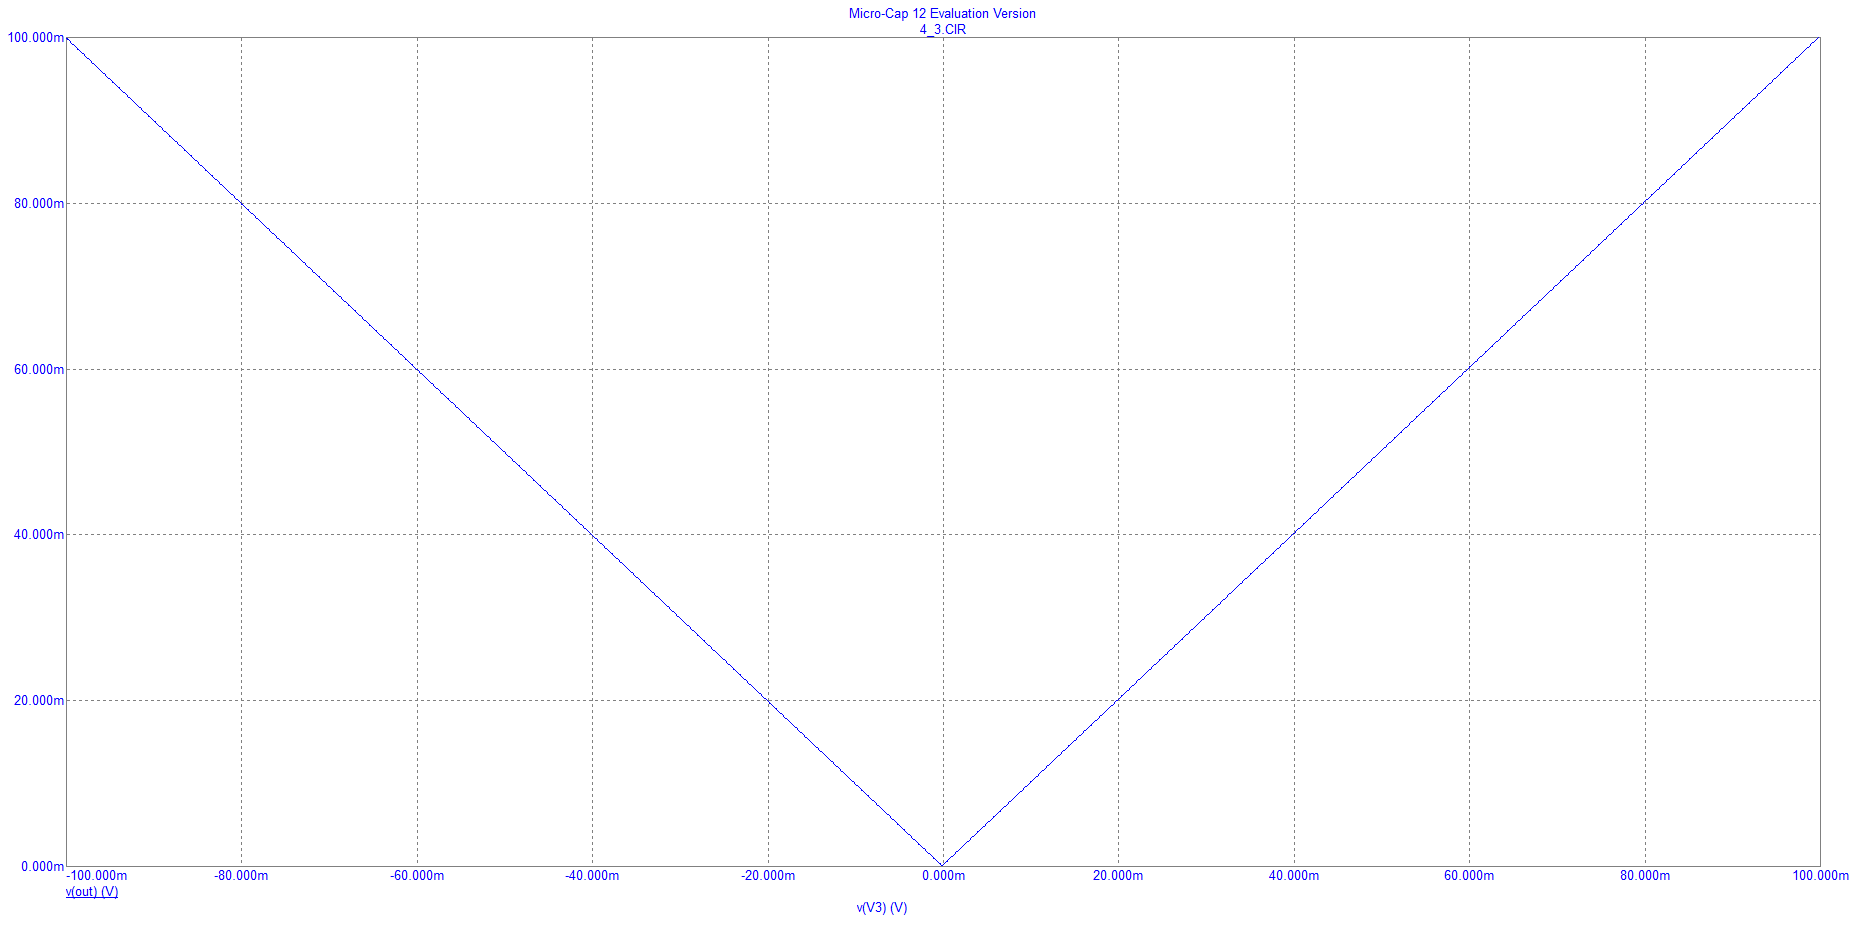
\includegraphics[width=0.8\textwidth]{microcap/3-dcprevodni.png}
    \caption{Zapojení c) -- stejnosměrná převodní charakteristika.}
    \label{fig:microcap/.png}
\end{figure}

\begin{figure}[h!]
    \centering
    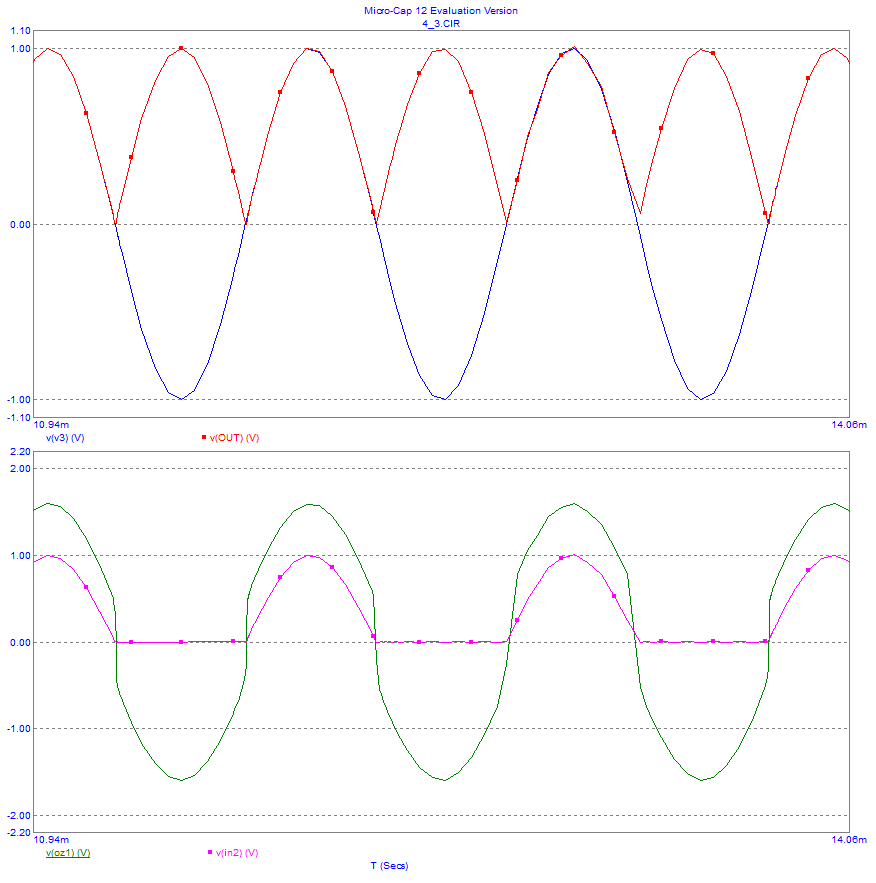
\includegraphics[width=0.66\textwidth]{microcap/3-transient-1khz-1v.png}
    \caption{Zapojení c) -- časová závislost napětí na výstupech obou OZ na vstupním napětí, jednocestné a dvoucestné usměrnění, \(f=\qty{1}{\kilo\hertz}, U_M=\qty{1}{\volt}\).}
    \label{fig:microcap/.png}
\end{figure}

\begin{figure}[h!]
    \centering
    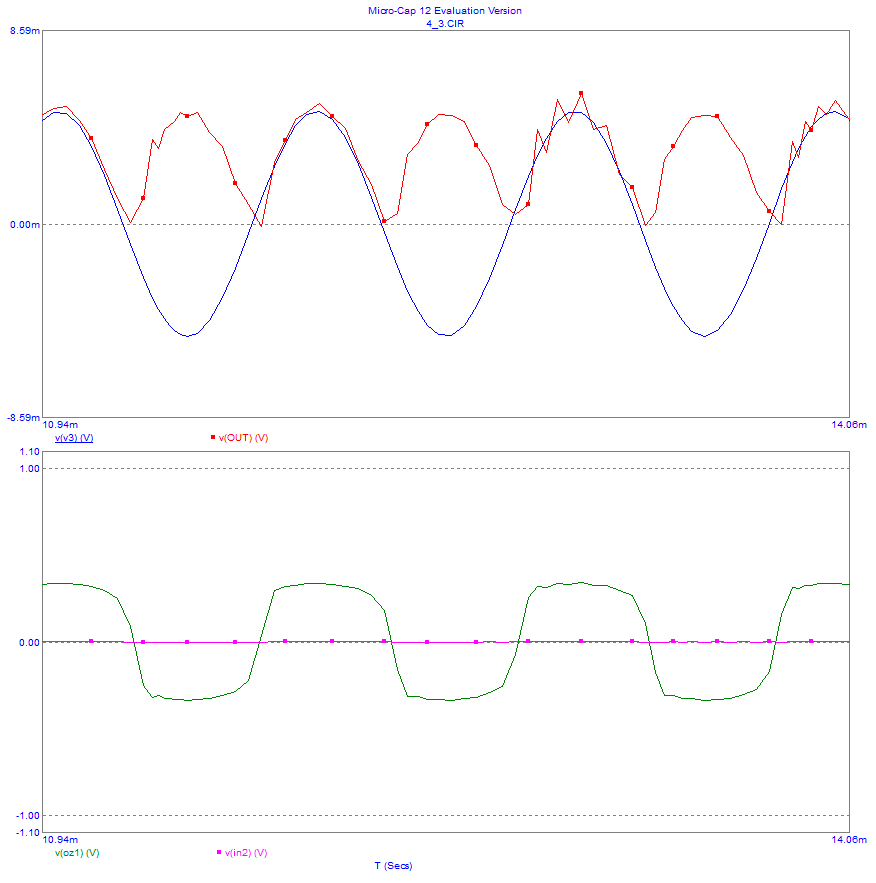
\includegraphics[width=0.66\textwidth]{microcap/3-transient-1khz-5mv.png}
    \caption{Zapojení c) -- časová závislost napětí na výstupech obou OZ na vstupním napětí, nejnižší amplituda, při které uspokojivě usměrňuje, \(f=\qty{1}{\kilo\hertz}, U_M=\qty{5}{\milli\volt}\).}
    \label{fig:microcap/.png}
\end{figure}

% \begin{figure}[h!]
%     \centering
%     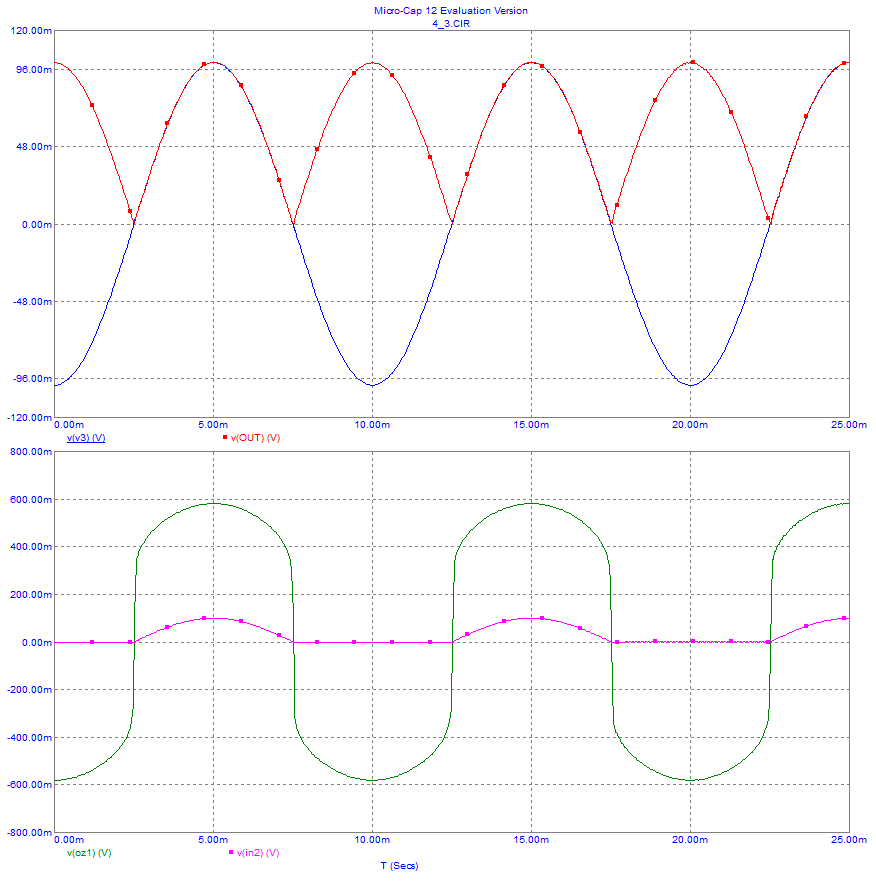
\includegraphics[width=0.8\textwidth]{microcap/3-transient-100hz-0.1v.png}
%     \caption{microcap/.png}
%     \label{fig:microcap/.png}
% \end{figure}

\begin{figure}[h!]
    \centering
    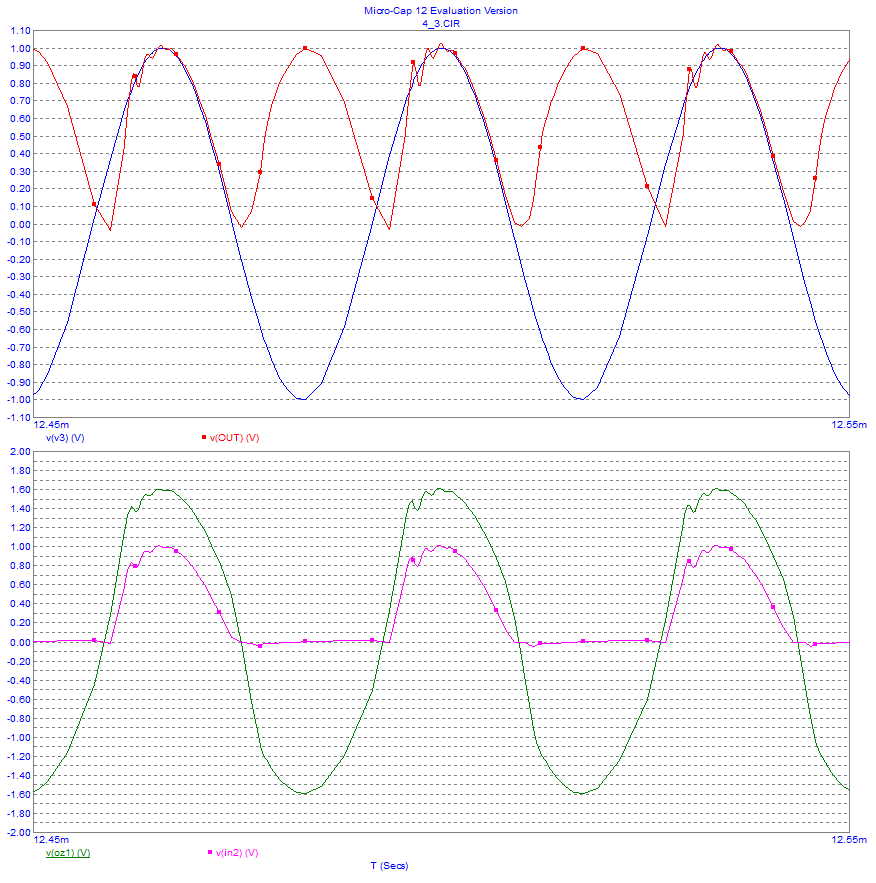
\includegraphics[width=0.8\textwidth]{microcap/3-transient-30khz-1v.png}
    \caption{Zapojení c) -- časová závislost napětí na výstupech obou OZ na vstupním napětí, nejvyšší frekvence, při které uspokojivě usměrňuje, \(f=\qty{30}{\kilo\hertz}, U_M=\qty{1}{\volt}\).}
    \label{fig:microcap/.png}
\end{figure}

